\section{Experimental Results}
\label{chap:ch4}

The verification of ACAS Xu benchmark involved evaluating the 10 properties against the 45 DNNs in the following manner: the first four were checked across all 45 networks, whereas the rest were checked on a single network. This approach followed the work done by the original authors \cite{10.1007/978-3-030-25540-4_26}. For each property, the timeout was set to 116 seconds. This verification process was performed using alpha-beta-CROWN and nnenum. Initially, the testing focused solely on property 1 against the first network to gain insights into the output. 

The output from alpha-beta-CROWN contains details about configuration, attack parameters, model output, properties, verification iterations, results, and a summary. Every iteration provides data about the batch size, the worst lower bound encountered, the total time spent in that iteration, the number of domains or branches explored, the cumulative time and the current lower bound - right-hand side value. This particular value is used to asses whether the property is satisfied or not, since a negative value indicates a potential violation of the property. One example of such iteration can be observed in figure \ref{Fig_It1}.

\begin{figure}[htbp]
	\centering
		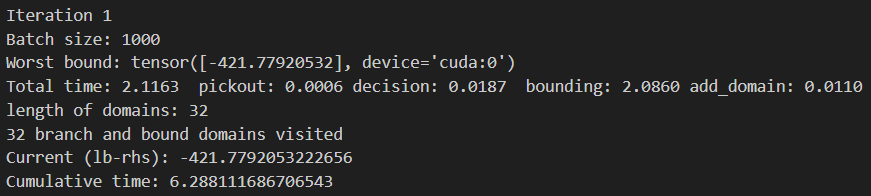
\includegraphics[width=14cm]{./Figures/it1.png}
	\caption{Alpha-Beta-CROWN first iteration in the verification process}
	\label{Fig_It1}
\end{figure}

In contrast to alpha-beta-CROWN, nnenum differs in that it produces more concise output, focusing primarily on the verification result and essential statistics such as runtime, work fraction completed, and the count of symbolic abstract states ('stars') evaluated. In the case of an unsafe result, a counterexample that demonstrates the violation is also shown. One such output is presented in figure \ref{Fig_Out1}.

\begin{figure}[htbp]
	\centering
		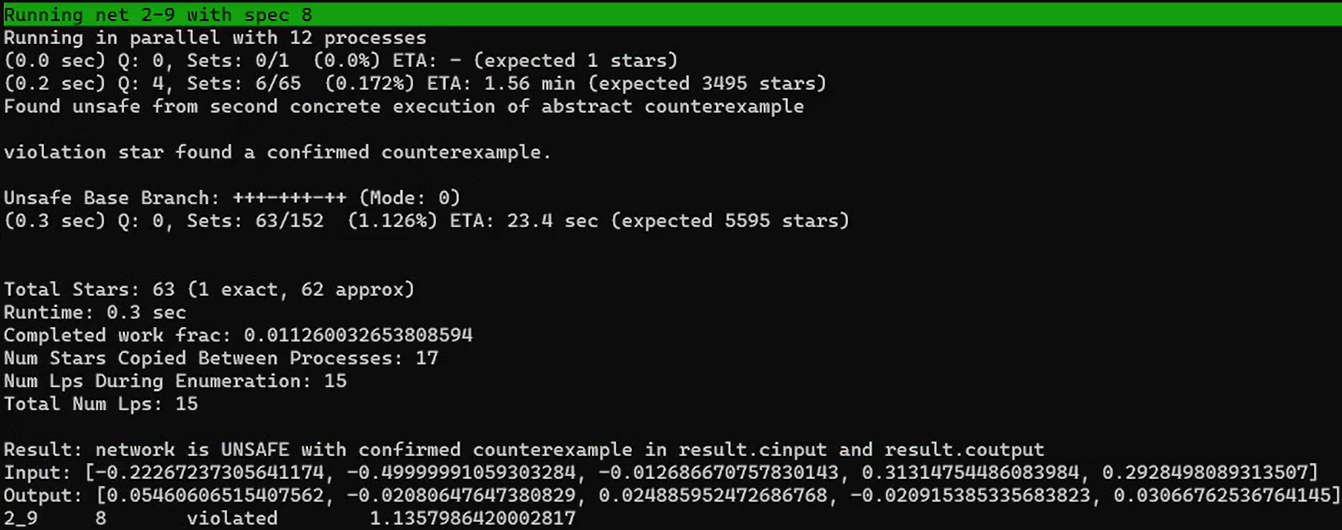
\includegraphics[width=14cm]{./Figures/nnenum_ex.png}
	\caption{nnenum unsafe output}
	\label{Fig_Out1}
\end{figure}

The next phase involved testing all properties, aiming to evaluate the neural network’s behavior across various configurations and constraints. The final verified accuracy stands at approximately 74.73\%. Upon comparing the results from alpha-beta-CROWN and nnenum for the 186 instances tested, both tools identified 139 instances as safe, meaning that the property held true, and 47 instances as unsafe. This information is summarized in table \ref{table:1}.

\begin{table}[h!]
\centering
\begin{tabular}{ |c c c c c| } 
\hline
Tool & Verified & Falsified & Penalty & Score \\
\hline
alpha-beta-CROWN & 139 & 47 & 0 & 1860 \\ 
nnenum & 139 & 47 & 0 & 1860 \\ 
\hline
\end{tabular}
\caption{Benchmark 2023-ACAS-Xu}
\label{table:1}
\end{table}

Regarding the verification times for alpha-beta-CROWN, the mean time taken for verifying all instances was approximately 2.58 seconds, with the maximum time being around 69.08 seconds. In terms of the employed methods, specifically the Branch and Bound method (BAB), 4 instances were marked as unsafe. In contrast, utilizing the Projected Gradient Descent (PGD) method, 47 instances were identified as unsafe.

As for nnenum, the performance achieved was quite similar, where all the instances have been verified, on average, in approximately 2.3 seconds with a maximum verification time of 61.58.

A more detailed overview is available on GitHub\footnote{\url{https://github.com/razvanmaciovan/Proiect-VF}}, featuring two CSV files that present results for both alpha-beta-CROWN and nnenum. These files detail the satisfiability and verification times for every tested combination. In addition, counter examples were generated and uploaded for the instances marked as unsafe.